%% ============================================================
%%  Major reframing plan
%%  (same template as draft.tex)
%% ============================================================
\documentclass[10pt,a4paper,fleqn]{article}
\setcounter{secnumdepth}{3}

\usepackage[margin=1in]{geometry}
\usepackage{graphicx}
\usepackage{float}
\usepackage{placeins}
\usepackage{xurl}
\usepackage{authblk}

\usepackage{CSPstyles}
\usepackage{tikz}
\definecolor{stimblue}{HTML}{5AB4E5}
\definecolor{stimorange}{HTML}{E6A700}
\usepackage{comment}
\usepackage{nicefrac}
\usepackage{times}
\usepackage{multicol}

\RequirePackage[style=authoryear-comp,
          natbib=true,
          hyperref=true,
          maxnames=3,
          doi=false,
          url=false,
          sortcites=false
          ]{biblatex}
\DeclareSourcemap{
  \maps[datatype=bibtex]{
    \map{
      \step[fieldset=abstract, null]
      \step[fieldset=annotation, null]
      \step[fieldset=annote, null]
    }
  }
}
\usepackage[final,
          colorlinks,
          linkcolor=black,
          citecolor=glaucous-main,
          urlcolor=glaucous-main,
          plainpages=false,
          pdfpagelabels,
          hypertexnames=false
          ]{hyperref}

%%% Bibliography %%%
\addbibresource{references.bib}
\setlength{\bibhang}{.125in}
\providecommand{\SortNoop}[1]{}

%========================================
% Packages
%========================================

\usepackage{amsmath}
\usepackage{amssymb}
\usepackage{booktabs}
\usepackage{subcaption}
\usepackage{enumerate}
\usepackage{paralist}
\usepackage{url}
\usepackage{setspace}
\usepackage{xspace}

% Packages required by the present manuscript.
\usepackage{tabularx}
\usepackage{multirow}
\usepackage{mathtools}
\usepackage{stmaryrd}
\usepackage{bm}
\usepackage{cleveref}
\usepackage{needspace}
\usepackage{todonotes}
\presetkeys{todonotes}{inline, backgroundcolor=yellow!40}{}
\graphicspath{{figures/}}

% Keep figures close to their first reference while allowing LaTeX to avoid
% large gaps around page boundaries.
\setcounter{topnumber}{4}
\setcounter{bottomnumber}{2}
\setcounter{totalnumber}{6}
\renewcommand{\topfraction}{0.90}
\renewcommand{\bottomfraction}{0.80}
\renewcommand{\textfraction}{0.08}
\renewcommand{\floatpagefraction}{0.70}

% ---- convenience commands ---------------------------------------------------
\newcommand{\eg}{\textit{e.g.}}
\newcommand{\ie}{\textit{i.e.}}
\newcommand{\adj}[1]{\textsc{#1}}
\newcommand{\utter}[1]{\textsf{#1}}
\newcommand{\param}[1]{\ensuremath{#1}}

% ---- title matter -----------------------------------------------------------
\title{Major Reframing Plan\\[1ex]
\normalsize New title: Disentangling Sources of Adjective Ordering in Referential Communication: From Conventionalised to Context-Specific Communicative Efficiency}
\author{}
\date{}

% =============================================================================
\begin{document}
\maketitle

\begin{abstract}
\noindent
Speakers across many languages prefer one order of adjectives over the others, and this preference has been explained by several sources, many of which share a notion of communicative efficiency.
Some of these sources, such as subjectivity, describe conventionalised efficiency at the level of the language, but are explained by an advantage in a particular referential context.
Under hierarchical composition with sequential context updating, placing the less subjective adjective closer to the noun helps the listener identify the intended object, and it has been suggested that even such a small advantage can accumulate into a convention over time.
Whether this advantage still plays a role each time a speaker produces an utterance, or whether speakers now simply follow the convention it has shaped, remains open.
It is also unclear how these sources interact with the choices specific to referential communication, in which speakers decide which adjectives to produce, often more than the context requires, and in which order to produce two or three of them.
Because the same surface order can result from different sources, we model production strategies in the Rational Speech Act framework and estimate the contribution of each source by comparing models with and without it.
The models are evaluated on two experiments on referential communication in German, a free production study and a slider rating study, in which the context-specific communicative efficiency of each adjective was manipulated.
The model comparisons show that the convention, represented by a stable order term, accounts for both which adjectives speakers select and the order in which they produce them.
Speakers respond to discriminatory strength, which stands for context-specific efficiency, mainly in which adjectives they produce, and adapt the order only gradually, as the slider ratings show, in which participants compare two orders directly.
Hierarchical composition helps to predict order only in models without the stable order term, which suggests that its advantage has become part of the convention rather than being computed anew in each context.
Finally, which adjectives speakers produce and their order differ in how far ahead speakers plan: looking ahead to the complete utterance captures which adjectives speakers produce, whereas producing them incrementally captures the order of two or three adjectives, so that a speaker model that combines both predicts the data better than a fully planned or a fully incremental one, which suggests that speakers plan their utterances partially.
\end{abstract}

\section{Introduction}

When several adjectives modify a noun, speakers across many languages prefer one order over the others; English speakers, for example, say \emph{the big blue sticker} rather than \emph{the blue big sticker} \citep{dixon1982,sproat1991,cinque1994,scott2002}.
This regularity has motivated a long tradition of research.
In an overview article, \citet{scontras2023adjective} summarises several sources, from intrinsic properties of adjectives, such as accessibility or subjectivity, to processing cost in comprehension and possibly also in production, and, last but not least, communicative success in specific contexts.
Recent work increasingly agrees that no single source alone accounts for the preferences.
\citet{dyer2023evaluating} found that, across 32 languages, combinations of predictors, such as subjectivity, frequency and length, predict adjective order better than any single predictor.
In another study on English, an account that combines subjectivity with collocation, the tendency of an adjective to be placed next to a noun with which it frequently occurs, outperforms each factor alone \parencites{futrell-etal-2020-determines}[see also][]{scontras2023adjective}.
Many of these sources share a similar notion of communicative efficiency, in that the preferred order either lowers the cost of processing a phrase or makes it more likely that the intended meaning gets across \citep{scontras2023adjective}.

These multi-factor analyses were carried out on corpora.
In such data, the target of explanation is the ordering preference that is already conventionalised in the language.
This preference is the end product of whatever pressures have shaped the language over time, not the pressures themselves.
What corpus studies show is which predictor, or which combination of predictors, explains the regularities at the level of the language well.
Moreover, some of the predictors are themselves defined at the level of the language, such as the frequency of an adjective \citep{dyer2023evaluating} or the mutual information between an adjective and a noun, that is, how much the occurrence of one tells about the occurrence of the other \citep{Hahn_information_2018}.
Such predictors are computed over all phrases in a corpus, so they describe the language rather than a particular speaker in a particular situation.
Here lies a problem of identifiability: the same surface order could result from different sources of pressure.
In some cases, several sources favour the same order, whereas in others they pull in opposite directions and the observed order nevertheless stays the same, which may be why no single factor wins, as the space of possible hypotheses behind each observed order is vast.
Studying corpora cannot disentangle these sources, because corpora offer no counterfactual comparison: they record the convention, and the utterances they contain are produced by speakers who have learnt it, so we never observe how the same speakers would order adjectives without it.

Some of the predictors, however, are motivated by cognitive explanations, which attribute an order to how speakers produce and how listeners understand language.
Take subjectivity as an example: in a corpus study and a rating study, \citet{scontras2017subjectivity} showed that more subjective adjectives are preferred farther from the noun.
This observation is again made at the level of the language, but the explanation is located in referential communication, in which a speaker describes one object so that a listener can identify it among others.
It has been argued that placing the less subjective adjective closer to the noun in the hierarchical structure reduces the risk that the listener misidentifies the intended object, because this adjective restricts the set of objects more reliably \citep{scontras2019grammatical}.
As a result, more subjective adjectives end up farther away from the noun.
\citet{franke2019subjectivity} showed in simulations that this account leads to a small advantage of the canonical order over the non-canonical order in communicative success, and suggested that even a small advantage can gradually strengthen into a convention.
\citet{scontras2023adjective} suggests extending this idea, that a small advantage in a particular referential context can accumulate over time, to the other efficiency-based predictors, and in doing so links two kinds of communicative efficiency: conventionalised efficiency at the language level and context-specific efficiency.
This link, however, has never been tested in referential communication, which raises the question of whether the pressure that may have shaped the convention still plays a role each time a speaker produces an utterance, or whether speakers now simply follow the convention it has shaped \citep{scontras2019grammatical}.

This question can be put to a test, because the explanations behind these sources name the situations in which one order should be preferred over another, and such situations can be created in controlled experiments in referential communication, where the efficient order can be made to differ from the conventional one.
Testing these sources in referential communication brings adjective order into another well-studied domain, the generation of referring expressions, which asks how speakers choose a description that identifies an object among others \citep{dale1995computational,van2019conceptualization}.
In this domain, one has to consider several aspects of the choice that corpora do not show.
First, speakers decide which properties of the object to mention at all \citep{van2019conceptualization}, so that order is only one part of the choice, as a speaker may produce a single adjective and then stop.
Second, speakers often mention more properties than needed to identify the object, and they use colour redundantly more often than size, which may be because colour is more salient \citep{tarenskeen2015overspecification,rubio2016redundant,degen2020redundancy}.
Both matter for ordering, because the former makes the order depend on which adjectives speakers produce: a speaker who starts with \emph{blue} can stop there, whereas a speaker who goes on has already decided which adjective comes first and is then unlikely to continue with size, given the canonical preference for size before colour.
The latter makes ordering a genuine problem, because redundant mention produces strings of multiple adjectives, whose possible orders have to be weighed against each other, even where a single adjective would identify the object.

Once redundant use has produced a string of multiple adjectives, the speaker still has to decide which of them comes first.
The most fundamental account of this decision problem is the incrementality efficiency hypothesis \citep{rubio2020incrementality,rubio2021wordorder}, as it makes direct predictions for ordering and places ordering at the centre of the investigation.
It starts from the observation that speakers produce and listeners interpret an utterance one word after another, so that a listener can already use the first adjective before the phrase is complete \citep{tanenhaus1995integration,sedivy1999achieving}.
Its predictions therefore concern which adjective a speaker should produce first, and two properties have been proposed to determine this, namely discriminatory strength, how well a property distinguishes the intended object from the other objects, and availability, how easily a property comes to the speaker's mind \citep{fukumura2018ordering}.
Incrementality and hierarchical composition can, however, make opposite predictions for the same context.
Under the incrementality efficiency hypothesis, the most discriminating adjective should come first, so that it narrows down the objects early \citep{fukumura2018ordering,rubio2021wordorder}, whereas under hierarchical composition, the adjective closest to the noun restricts the objects first, so that the adjective that restricts them most reliably should come last \citep{scontras2019grammatical,franke2019subjectivity}.
Because the two accounts assume a different underlying structure, what counts as efficient ends up in different surface orders.
How do speakers reconcile this tension?
Do they nevertheless follow the convention, or do they adapt the order to the communicative efficiency in the particular context?

Referential communication is thus where conventionalised and context-specific communicative efficiency meet, but the two lines of work have so far been studied apart.
Accounts of the convention have been tested on corpora and in simulations, whereas studies of referring expressions have examined one or two context-specific pressures at a time, so that their contributions have not been estimated together with that of the convention.
Studies of adjective ordering in referential communication have even deliberately avoided the convention: \citet[p.~39]{fukumura2018ordering} studied colour and pattern instead of size and colour, because the latter preference may be ``too conventionalized to be easily overridden by communicative and cognitive constraints''.
What is missing is a multi-factor analysis of adjective order in referential communication, comparable to the analyses of corpora described above, in which the sources proposed for the language level and those proposed for the context-specific level are evaluated on the same dataset in a unified modelling framework.
Such an analysis requires, first, controlled experiments instead of corpora, in which, as argued above, the order that is efficient in a particular context can be made to differ from the conventional one.
This targets directly the question of whether speakers adapt the order to the context or simply follow the convention.
Second, controlled experiments alone do not suffice, and this is what has made the link between conventionalised and context-specific communicative efficiency difficult to test so far: even in a controlled experiment, the problem of identifiability remains, as the same surface order can result from different sources, and the convention is present in every display.
This is where cognitive modelling becomes useful: it can disentangle the stable ordering convention from the other sources by representing it as a component of its own, and it can map each source explicitly to a model variant that includes it.
This mapping can even be made at the algorithmic level, so that, for example, questions about sequential context updating and incremental production can be asked by implementing them.
Such models link theories to data: a source such as hierarchical composition states which order is efficient, but not how often speakers produce each utterance in a given display, and a probabilistic model of language use turns it into such quantitative predictions, which can be compared with what participants actually produce \citep{franke2016task,van2021probabilistic}.
Moreover, once the convention is represented in this way, the contribution of each source to a surface order that is otherwise unidentifiable can be estimated by matched model comparisons, in which two models differ in only one source while the convention and the other sources are kept in place, as showcased by other studies that used probabilistic pragmatic models \citep{franke2016reasoning,van2021probabilistic,franke2016probabilistic}.
We consider a space of a priori plausible production strategies, in which each source is either present or absent, and compare them with one another.
We therefore ask what role these sources play in adjective ordering in referential communication, and how much each of them contributes.

To answer this question, we build production models within the Rational Speech Act framework \citep{frank2012predicting,goodman2016pragmatic}.
Each source is formalised as a separate component of the model.
The convention is represented by a stable order term, which stands for conventionalised efficiency and favours the orders that are frequent in German text, as estimated by a pre-trained language model, in the same way in every display.
This term thus covers all language-level sources together, including the mutual information between adjectives and nouns proposed by information-theoretic accounts \citep{Hahn_information_2018,futrell-etal-2020-determines}, without distinguishing between them.
Hierarchical composition is implemented by sequential context updating, under which each adjective is interpreted among the objects that the adjectives closer to the noun have selected, whereas under context-fixed semantics every adjective is interpreted among all objects in the display.
If the reasoning behind composition is still carried out in each context, sequential context updating should improve the prediction of order.
Discriminatory strength is implemented as informativeness, which values an adjective by how well it identifies the intended object in the display, and availability as salience, which combines a fixed preference for each property, higher for colour than for size and form, with how strongly the property stands out from the other objects in the display.
Incrementality is implemented by the degree of planning, that is, how far ahead the speaker evaluates an utterance \citep{cohngordon2019incremental,waldon2021modeling}.
A global speaker evaluates only complete utterances, a fully incremental speaker evaluates each adjective as it is produced without looking ahead, and an intermediate speaker evaluates each adjective as it is produced while looking ahead to the complete utterance.
The intermediate speaker implements partial planning: if production is good enough, speakers begin to speak before every part of an utterance has been planned, but they still plan some of it in advance \citep{ferreira2002incremental,ferreira2002goodenough}.

We also report two experiments with German speakers in a reference game setting, in which the context-specific communicative efficiency of each adjective was manipulated.
In a production study, participants freely chose what to say, which is a natural task for probing the full distribution of possible utterances, to which the models are fitted.
This distribution reflects which adjectives speakers produce, as they may produce a single adjective or more adjectives than the context requires, and the order of two or three adjectives.
In a slider study, by contrast, participants rated their preference between two competing orders.
After the models are fitted to the production data, they are evaluated on both datasets using matched model comparisons.
The main measure is the gain in out-of-sample predictive accuracy when a source is added to a model, together with how well the model generalises to the slider task, on which it was not fitted.
Section~\ref{sec:setup} introduces the models and the experimental design, Section~\ref{sec:experiments} reports the experiments, Section~\ref{sec:results} presents the model comparisons, and Section~\ref{sec:conclusion} concludes.

\section{Study setup: models and experiments}
\label{sec:setup}

The production models formalise each source of ordering preference described above as a separate component, and the experiments vary the referential context so that these components favour different utterances.
We introduce both at the level needed to follow the model comparisons, while the formal specification of the models appears in \Cref{app:model} and the experiments are described in \Cref{sec:experiments}.

The models are defined over the displays and descriptions of the production experiment.
The states are the six objects of a display, among which the target $o^*$ is the intended referent, and each object is represented by its size, colour and form.
The utterances are the fifteen adjective strings coded in the experiment, which contain one, two or three of the adjectives for size, colour and form, in every possible order.
Size has a threshold-based meaning, under which an object counts as \emph{big} to the degree that its size exceeds a threshold set by its comparison class \citep{schmidt2009how,franke2019subjectivity}, whereas colour and form have relaxed meanings, under which the objects of the named colour or form receive most, but not all, of the weight \citep{degen2020redundancy}.
The literal interpretation $L$, which corresponds to the literal listener of RSA models, composes the adjectives of a string hierarchically from the noun outwards, so that in \emph{big blue sticker}, \emph{blue} modifies \emph{sticker} before \emph{big} is interpreted.

All model variants are instances of one speaker, who chooses an utterance $u=w_1\ldots w_T$ for the target $o^*$ in the display $C$ with probability
\begin{equation}
  S(u\mid o^*,C)
  \propto
  S_{\mathrm{G}}(u\mid o^*,C)^{\,1-\kappa}\;
  S_{\mathrm{I}}(u\mid o^*,C)^{\,\kappa},
  \qquad
  \underbrace{0\le\kappa\le1}_{\substack{\text{interpolation}\\[1pt]\text{global}\,\leftrightarrow\,\text{incremental}}},
  \label{eq:full-speaker}
\end{equation}
which interpolates between a global speaker, who compares complete utterances,
\begin{equation}
  S_{\mathrm{G}}(u\mid o^*,C)
  \propto
  \exp\Bigl\{
  \underbrace{\beta\,\Omega(u)}_{\substack{\text{stable order term}\\[1pt]\text{conventionalised}\\[1pt]\text{efficiency}}}
  \;-\;\underbrace{c(u)}_{\substack{\text{utterance}\\[1pt]\text{cost}}}
  \;+\;\sum_{t} U(w_{t+1}\mid w_{1:t})
  \Bigr\},
  \label{eq:global-speaker}
\end{equation}
and a fully incremental speaker, who chooses each adjective among those still available at its position,
\begin{equation}
  S_{\mathrm{I}}(u\mid o^*,C)
  \propto
  \exp\bigl\{\beta\,\Omega(u)-c(u)\bigr\}
  \prod_{t}
  \frac{\exp U(w_{t+1}\mid w_{1:t})}{\sum_{w'}\exp U(w'\mid w_{1:t})}.
  \label{eq:incremental-speaker}
\end{equation}
Both speakers value each adjective by its utility at its position in the utterance,
\begin{equation}
  U(w_{t+1}\mid w_{1:t})
  =
  \underbrace{\alpha\log L_{C_t}(o^*\mid w_{1:t+1})}_{\mathclap{\substack{\text{informativeness}\\[1pt]\text{discriminatory strength}}}}
  +\underbrace{\lambda\,z_{w_{t+1}}}_{\mathclap{\substack{\text{salience}\\[1pt]\text{availability}}}},
  \label{eq:adjective-utility}
\end{equation}
where the adjectives are interpreted against the set of objects
\begin{equation}
  \underbrace{C_t=C\ \ \text{(context-fixed)}\quad\text{or}\quad C_t=L_{t+1}\ \ \text{(sequential context updating)}}_{\text{hierarchical composition}}.
  \label{eq:comparison-class}
\end{equation}
Here $L_{C_t}(o^*\mid w_{1:t+1})$ is the probability that the adjectives produced so far, interpreted from the noun outwards, pick out the target, and $C_t$ is the set of objects against which each adjective is interpreted.
The first term of the utility thus implements discriminatory strength, valuing an adjective by how well it identifies the target at its position, with $\alpha$ setting how strongly the speaker attends to it.
Because this value is summed over the positions of an utterance, an utterance gains value when it identifies the target early, not only when it is complete.
The second term implements availability, following the observation that visually salient properties, colour in particular, are often mentioned even when they are redundant \citep[p.~2]{rubio2016redundant}, and that more salient properties tend to be produced earlier \citep[p.~47]{fukumura2018ordering}.
The salience score $z_w$ combines a fixed preference for each property, higher for colour than for size and form, with how strongly the target differs in that property from the other objects in the display, and $\lambda$ sets how much the speaker prefers to produce salient properties early.

Under context-fixed semantics the set $C_t$ is the whole display, whereas under sequential context updating it is the set of objects that the adjectives closer to the noun have selected.
Consider a display in which the target is a medium-sized blue object, the other blue objects are small, and the red objects are larger than the target.
Against the whole display, the target is not particularly big, so \emph{big} applies more strongly to the red objects.
In \emph{big blue}, however, \emph{blue} is interpreted first, and under sequential context updating \emph{big} is then judged among the blue objects, among which the target is the largest.
In \emph{blue big}, by contrast, \emph{big} is next to the noun and is interpreted against the whole display.
Sequential context updating can therefore make the size-first order more informative than the colour-first order, as proposed by hierarchical composition \citep{scontras2019grammatical,franke2019subjectivity}, whereas under context-fixed semantics both orders receive the same interpretation.

The two remaining components are added to the summed utilities of the complete utterance.
The stable order term $\beta\Omega(u)$ weights a fixed score $\Omega(u)$ for the order of the adjectives in $u$, derived from a pre-trained German language model, so it favours the orders that are frequent in German text in the same way in every display.
\citet[p.~124]{schlotterbeck2023incremental} found a strong preference for size-first order in slider ratings, and our replication found this preference even when colour alone identified the target (\Cref{sec:experiments}).
The utterance cost $c(u)$, which here also covers preferences for how many and which adjectives speakers produce, is an auxiliary component that links the model to the task \citep{lee2013bayesian,franke2016task}.
It is present in every variant and does not stand for a theory of ordering.

The parameter $\kappa$ sets how far ahead the speaker evaluates an utterance: $\kappa=0$ gives the global speaker, $\kappa=1$ the fully incremental speaker, and values in between an intermediate speaker, who plans the utterance partially, evaluating each adjective as it is produced while looking ahead to the complete utterance.
The two endpoints differ in whether the adjectives that follow can compensate for a first adjective whose utility is low relative to its competitors.
In a colour-sufficient display, where \emph{blue} alone identifies the target, the global speaker evaluates the prefix \emph{big} only as one part of the summed utility of \emph{big blue}, which is compared with the other complete utterances.
The fully incremental speaker, by contrast, must first choose \emph{big} over \emph{blue} at the first position, where \emph{blue} identifies the target on its own and \emph{big} does not, and the later adjectives cannot offset this choice.
At intermediate values of $\kappa$, the utility of \emph{blue} after \emph{big} offsets the low utility of \emph{big} only in part, so that the speaker can keep the conventional order \emph{big blue}, while the competition from \emph{blue} at the first position makes colour-initial utterances more likely than under global production.
Speakers may differ in how far ahead they plan, so we also consider a speaker in which each participant $i$ has a value $\kappa_i$, drawn from a distribution shared by all participants.

Each source is tested by a matched comparison that removes one component and keeps the others in place, setting $\beta=0$ for the convention, $\alpha=0$ for discriminatory strength and $\lambda=0$ for availability, or replacing sequential context updating by context-fixed semantics for hierarchical composition.
The parameters of all components are estimated jointly from the production data, and the fitted models then predict the slider ratings without being refitted.

Both experiments used a reference game about collectible stickers, in which participants saw six objects, one of them framed as the target, and described it so that a partner, who saw the same objects in a different order and without the frame, could identify it (\Cref{fig:schematic}).
Referential context, manipulated within participants, varied the context-specific efficiency of each adjective by determining whether size alone (size sufficient), colour alone (colour sufficient) or both properties (both necessary) identified the target.
In colour-sufficient displays, the order that is efficient in the context differs from the conventional one, as discriminatory strength favours beginning with \emph{blue}, whereas the convention favours \emph{big blue}.
Size discriminability, manipulated between participants, varied how clearly the size difference between the target and its competitor could be seen.
Each context was realised with three adjective pairs, size--colour, size--form and colour--form, so that size and colour were not always the properties that distinguished the target.
In the production study, participants completed the sentence frame \emph{den \ldots\ Aufkleber} (`the \ldots\ sticker') freely, whereas in the slider study they rated their preference between the two orders of the same two adjectives.

\begin{figure}[htbp]
\centering
\begin{tikzpicture}[
  obj/.style={circle, draw=black!70, line width=0.4pt, inner sep=0pt},
  blu/.style={obj, fill=stimblue},
  org/.style={obj, fill=stimorange},
  target/.style={draw=red!80!black, line width=1pt},
  lab/.style={font=\small\bfseries, anchor=west},
  note/.style={font=\footnotesize, align=center},
  panel/.style={draw=black!25, rounded corners=2pt, fill=black!3}
]
% ---------- Panel A: referential context ----------
\node[lab] at (-0.2,3.15) {A\quad Referential context (within participants)};
\foreach \x/\title/\note in {0/{size sufficient}/{distinguishing property: size},
                             5.4/{colour sufficient}/{distinguishing property: colour},
                             10.8/{both necessary}/{size and colour needed}}{
  \draw[panel] (\x,0.05) rectangle ++(4.9,2.65);
  \node[note, anchor=north] at (\x+2.45,2.62) {\textit{\title}};
  \node[note, anchor=south] at (\x+2.45,0.12) {\note};
  \draw[target] (\x+0.35,0.95) rectangle ++(1.0,1.0);
}
% objects: target first, then three competitors
\node[blu, minimum size=8.5mm] at (0.85,1.45) {};
\node[blu, minimum size=4.5mm] at (2.05,1.45) {};
\node[org, minimum size=4.5mm] at (3.15,1.45) {};
\node[org, minimum size=4.5mm] at (4.20,1.45) {};
\node[blu, minimum size=8.5mm] at (6.25,1.45) {};
\node[org, minimum size=8.5mm] at (7.45,1.45) {};
\node[org, minimum size=4.5mm] at (8.55,1.45) {};
\node[org, minimum size=4.5mm] at (9.60,1.45) {};
\node[blu, minimum size=8.5mm] at (11.65,1.45) {};
\node[blu, minimum size=4.5mm] at (12.85,1.45) {};
\node[org, minimum size=8.5mm] at (13.95,1.45) {};
\node[org, minimum size=4.5mm] at (15.00,1.45) {};
% ---------- Panel B: size discriminability ----------
\node[lab] at (-0.2,-0.35) {B\quad Size discriminability (between participants)};
\draw[panel] (0,-2.6) rectangle ++(7.6,2.0);
\node[blu, minimum size=8.5mm] at (1.0,-1.55) {};
\draw[target] (0.5,-2.05) rectangle (1.5,-1.05);
\node[blu, minimum size=4.5mm] at (2.2,-1.55) {};
\node[note] at (1.6,-2.35) {high: large size gap};
\node[blu, minimum size=8.5mm] at (4.6,-1.55) {};
\draw[target] (4.1,-2.05) rectangle (5.1,-1.05);
\node[blu, minimum size=7mm] at (5.8,-1.55) {};
\node[note] at (5.2,-2.35) {low: small size gap};
% ---------- Panel C: tasks ----------
\node[lab] at (8.0,-0.35) {C\quad Tasks};
\draw[panel] (8.2,-2.6) rectangle ++(7.5,2.0);
\node[note, anchor=west] at (8.4,-1.1) {\textbf{Production:} den \underline{\hspace{1.6cm}} Aufkleber};
\node[note, anchor=west] at (8.4,-1.55) {free choice of adjectives and their order};
\node[note, anchor=west] at (8.4,-2.05) {\textbf{Slider:} \emph{big blue}};
\draw[black!60, line width=0.6pt] (10.95,-2.05) -- (13.45,-2.05);
\fill[black!70] (12.6,-2.05) circle (1.6pt);
\node[note, anchor=west] at (13.55,-2.05) {\emph{blue big}};
\node[note, anchor=west] at (8.4,-2.4) {preference between two given orders};
\end{tikzpicture}
\caption{Schematic display and manipulated factors, shown for the size--colour pair; the framed object is the target.
(A) The referential context determines which property distinguishes the target, so that the order that is efficient in the context can agree with the conventional order \emph{big blue} (size sufficient) or differ from it (colour sufficient).
(B) Size discriminability varies the size gap between the target and the competitor of the same colour.
(C) In the production study participants complete the sentence frame freely, whereas in the slider study they rate their preference between two given orders.
The size--form and colour--form pairs follow the same scheme.}
\label{fig:schematic}
\end{figure}

\section{Experiments}
\label{sec:experiments}

I think it is valuable to bring the slider study back.
Most importantly, competing orders are rare in production, so the production dataset is first about separating selection from ordering, and ordering then depends on selection.
If the main story is about ordering and the different theories around it, the slider study can be insightful, because it forces a comparison between two orders and shows how the preference changes gradually with the context.
Practically, it is cool to train the models on one dataset and evaluate them on another.
Second, we already did the replication! so including the slider study makes the most of what we have.
We also get a clear story about our own earlier study by referring back to FW2023, as we can say that the present models are similar to that model in spirit but differ from it.

Reporting the results can be short, and hypothesis testing can be minimal, as they are not central to the main thread.

\section{Model Comparison Results}
\label{sec:results}

\subsection{Best-fitting model}
\label{sec:best}

The best-fitting model is an intermediate speaker, with $\kappa$ between the global and the fully incremental speaker (Equation~\ref{eq:full-speaker}), context-fixed semantics, the stable order term, informativeness and salience.
This speaker evaluates each adjective as it is produced while looking ahead to the complete utterance, follows the conventional order, values adjectives that identify the target in the display, and prefers to mention colour.
The model predicts the production data well, as the predicted proportion of each utterance in each display closely follows the observed proportion (Figure~\ref{fig:best}).
We therefore use this model as the reference for the matched contrasts below: because it describes the data well, each contrast removes one component from a model that captures the data, and the difference it yields can be read as the contribution of that component rather than as a misfit of the reference model.

\begin{figure}[H]
\centering
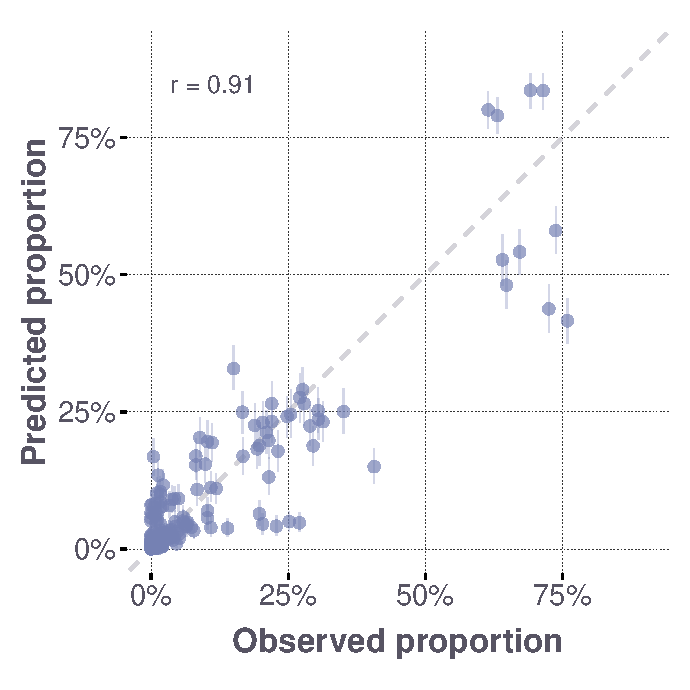
\includegraphics[width=.5\textwidth]{figures/best_model_fit.pdf}
\caption{Observed against predicted proportions of each utterance in each display for the best-fitting model; error bars show 95\% posterior predictive intervals.}
\label{fig:best}
\end{figure}

\subsection{Overview of the matched contrasts}

First, here is an overview figure that covers both tasks (production and slider ratings), the four sources, and both which adjectives speakers produce and their order.
Every contrast compares two models that differ in one component, starting from the best-fitting model as the reference model.
Model A contains the component that a theoretical claim refers to, model B is the alternative, and all values are A minus B.
In production, the value is the difference in expected log predictive density (ELPD), given separately for which adjectives speakers produce and for the order of two or three adjectives, so that a positive value means that A predicts the produced utterances better.
In the ratings, the production models are not refitted: each model predicts, for every display, the preference for the conventional order, for example \emph{big blue} over \emph{blue big}, and we ask how well these predictions fit the observed ratings.
The value is the $R^2$ of A minus the $R^2$ of B, so that a positive value again means that A predicts the data better.

\begin{figure}[H]
\centering
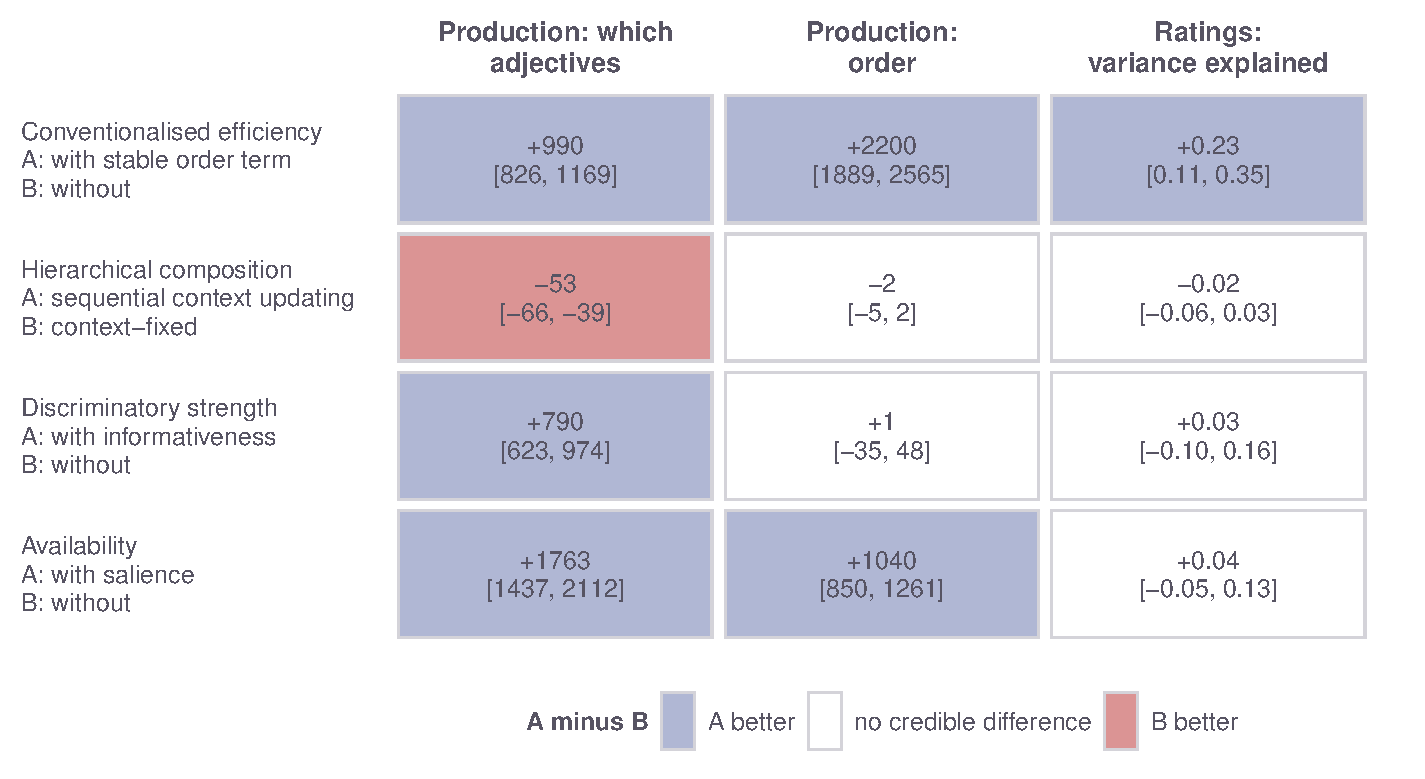
\includegraphics[width=\textwidth]{figures/reframing_overview.pdf}
\caption{Overview of the model contrasts.
Each row is one theoretical claim with the two models that test it, and each column is one measure.
Cells give A minus B with 95\% credible intervals, as a difference in ELPD for production and as a difference in $R^2$ for the ratings; blue cells favour A, red cells favour B, and white cells show no credible difference.
All contrasts are shown for the intermediate speaker; the contrasts with the global and the fully incremental speaker are shown in Figure~\ref{fig:architecture}.}
\label{fig:overview}
\end{figure}

\subsection{Conventionalised efficiency}

The stable order term improves the prediction of which adjectives speakers produce and of their order in production for all three speakers, and in the ratings it improves prediction for the intermediate and the fully incremental speaker but not for the global speaker (Figure~\ref{fig:infotheory}).
The global speaker without the stable order term predicts the ratings best, because its predictions vary only with the informativeness of the complete phrase in the display, which is what participants compare when both orders are given side by side, whereas the stable order term adds differences between adjective pairs that are larger than those in the ratings.
For the accounts at the language level, this means that the order speakers produce follows a convention that is the same in every display, and the stable order term does not distinguish the information-theoretic accounts \citep{Hahn_information_2018,futrell-etal-2020-determines} from conventionalised composition as its source.

\begin{figure}[H]
\centering
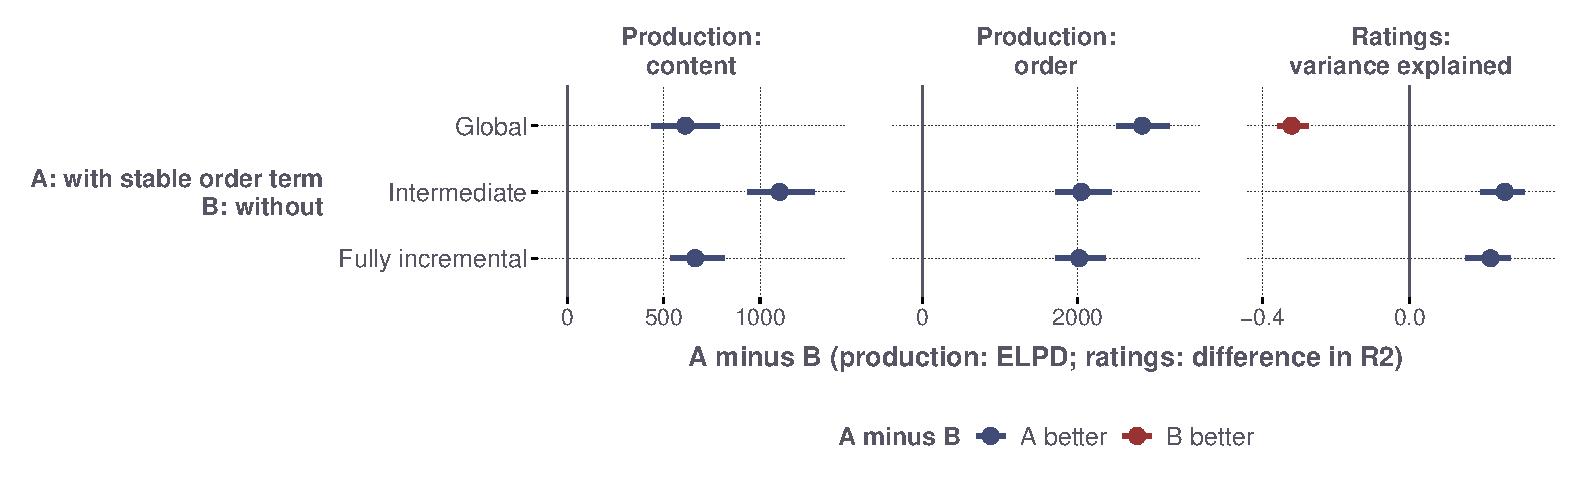
\includegraphics[width=\textwidth]{figures/reframing_zoom_lexical.pdf}
\caption{Conventionalised efficiency: models with and without the stable order term, for the global, intermediate and fully incremental speaker.}
\label{fig:infotheory}
\end{figure}

\subsection{Hierarchical composition}

Sequential context updating adds no predictive benefit to production or to the prediction of the ratings (Figure~\ref{fig:composition}).
However, removing the stable order term reveals a reversal: for the global speaker, sequential context updating then improves the prediction of order in production.
Hierarchical composition thus predicts order only for a speaker who evaluates the complete utterance and has no convention to rely on, which is the setting in which it was proposed \citep{scontras2019grammatical,franke2019subjectivity}.
In other words, it does the same job as the stable order term, although with a much smaller effect.
That is, although we found no benefit of hierarchical composition for referential communication when the stable order term is included, we also found evidence that hierarchical composition can compensate for the stable order term, which supports it as an explanation of how this convention arose.

\begin{figure}[H]
\centering
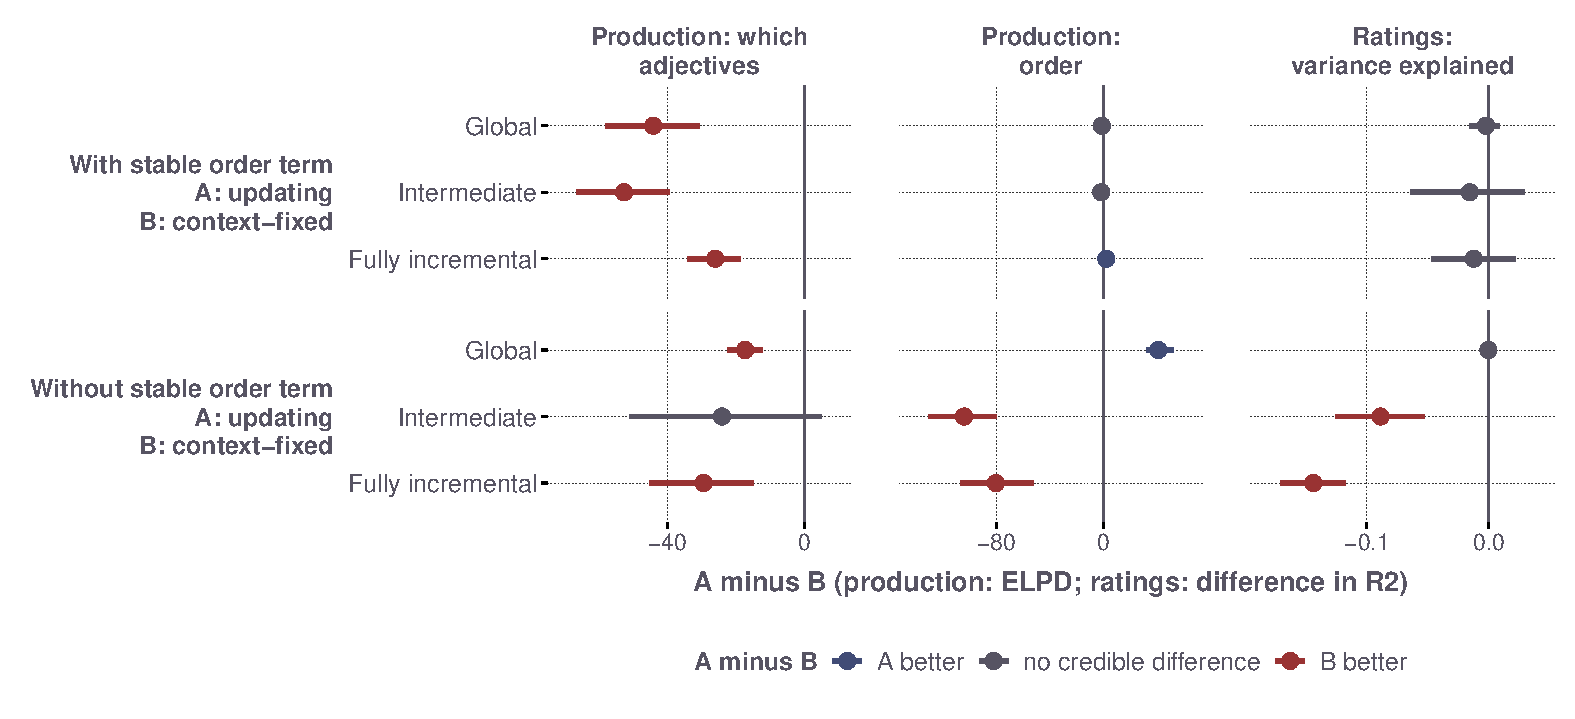
\includegraphics[width=\textwidth]{figures/reframing_zoom_composition.pdf}
\caption{Hierarchical composition: sequential context updating against context-fixed semantics, with and without the stable order term, for the global, intermediate and fully incremental speaker.}
\label{fig:composition}
\end{figure}

\subsection{Discriminatory strength}

Discriminatory strength (i.e.\ informativeness) mainly improves the prediction of which adjectives speakers produce for all three speakers, that is, the first adjective and whether speakers stop after it, but for order, it has a little to no benifit. (Figure~\ref{fig:incremental}).
This means, people resolving the pressure from referential context mainly by which adjectives they produce. And if people do ordering, then this goes in the direction of more discriminating property first, as showed by rating data.

\begin{figure}[H]
\centering
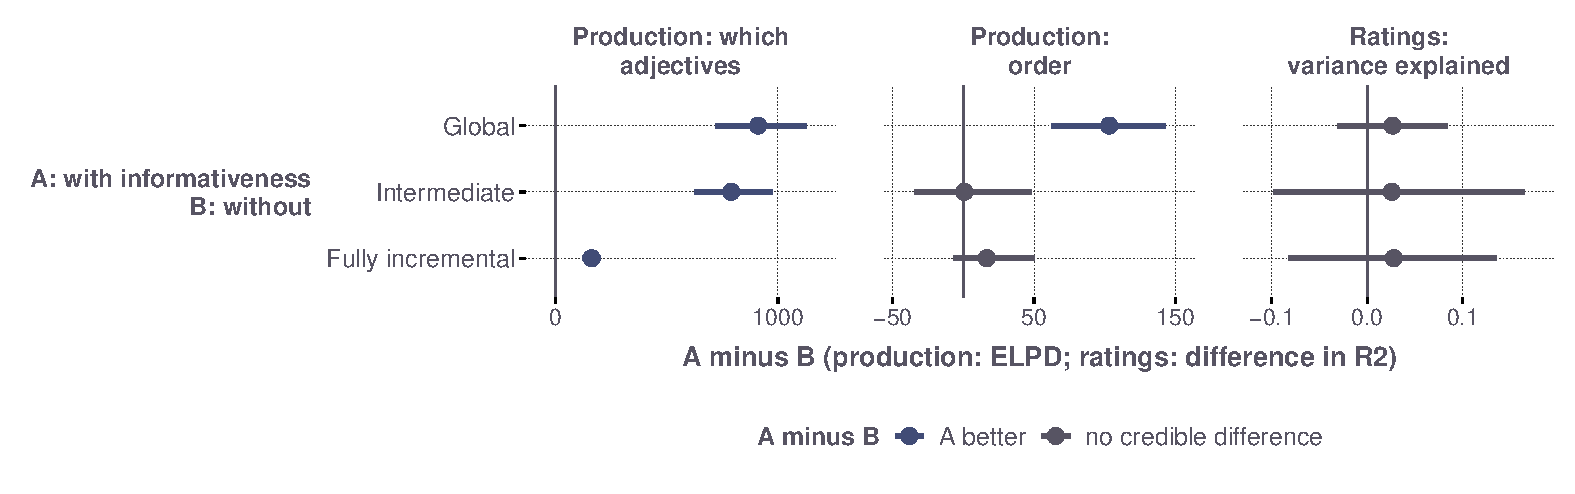
\includegraphics[width=\textwidth]{figures/reframing_zoom_incremental.pdf}
\caption{Discriminatory strength: models with and without informativeness, for the global, intermediate and fully incremental speaker.}
\label{fig:incremental}
\end{figure}

\subsection{Availability}

Salience improves the prediction of both which adjectives speakers produce and their order in production for all three speakers, which is similar to what \citet{fukumura2018ordering}.
However, salience does not improve the prediction of the ratings for the intermediate speaker.
This is because, in the model, salience is an intrinsic property of colour and form, which remains the same in every display, so the availability of a property \citep{fukumura2018ordering} acts here as a stable preference for mentioning it early and does not adapt to the referential context.
Such a preference only adds differences between adjective pairs, and these are larger than the differences in the ratings, as for the stable order term.

\begin{figure}[H]
\centering
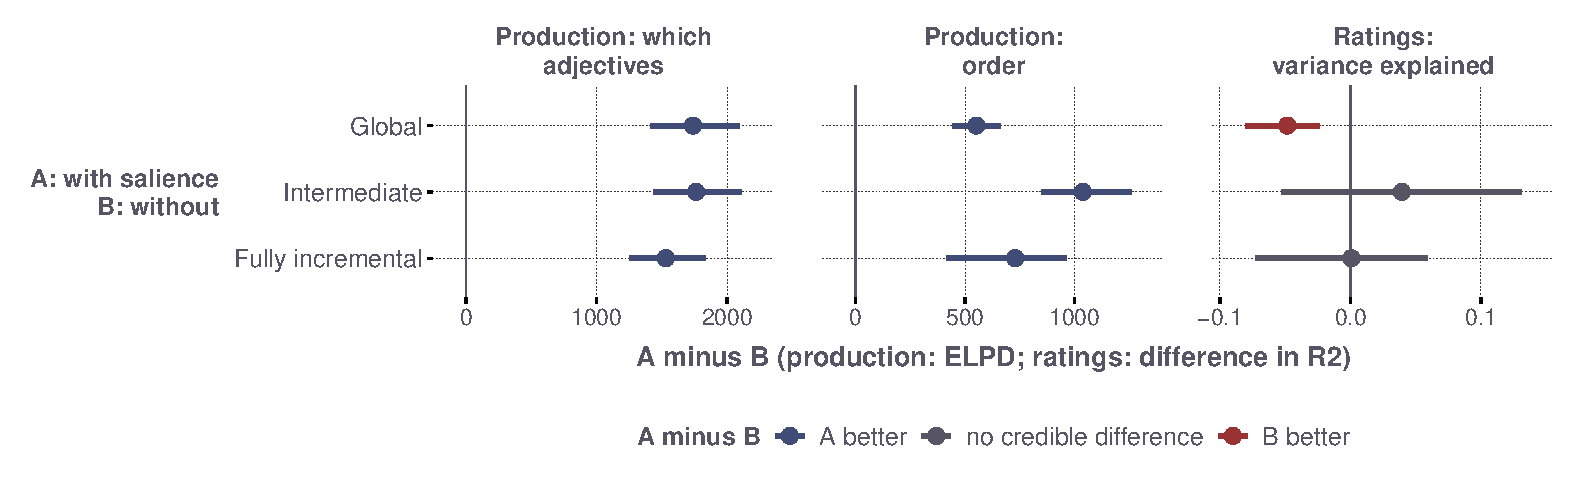
\includegraphics[width=\textwidth]{figures/reframing_zoom_availability.pdf}
\caption{Availability: models with and without salience, for the global, intermediate and fully incremental speaker.}
\label{fig:availability}
\end{figure}

\subsection{Partial planning}
The contrasts of the intermediate speaker with the global speaker ($\kappa=0$) and the fully incremental speaker ($\kappa=1$) show how the interpolation behaves: it predicts order better than the global speaker and which adjectives speakers produce better than the fully incremental speaker.
Evaluating each adjective as it is produced, which separates the intermediate from the global speaker, improves order in production, whereas looking ahead to the complete utterance, which separates it from the fully incremental speaker, improves which adjectives speakers produce, and the three speakers predict the ratings about equally well (Figure~\ref{fig:architecture}).
This places speakers between the global speaker assumed in the composition accounts and a fully incremental speaker, as expected if production is good enough and only partially planned \citep{ferreira2002incremental,ferreira2002goodenough}.

\begin{figure}[H]
\centering
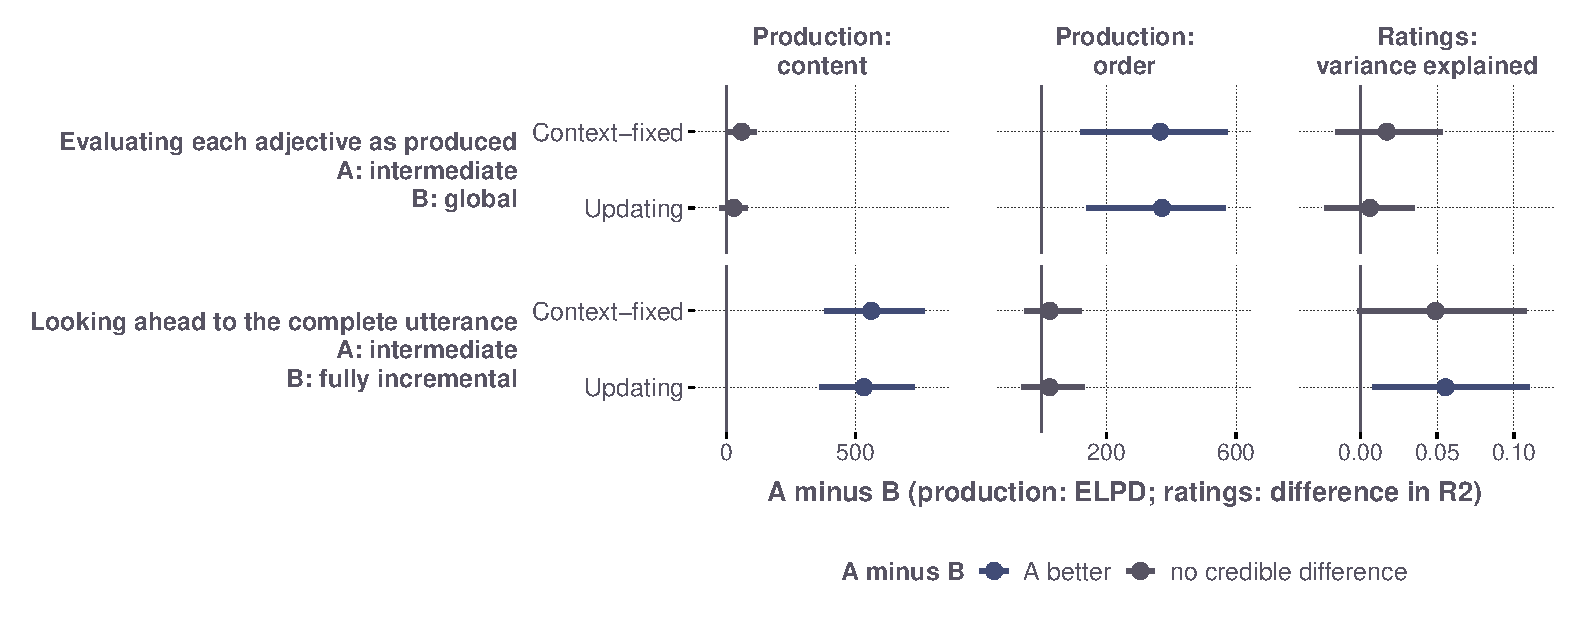
\includegraphics[width=\textwidth]{figures/reframing_zoom_architecture.pdf}
\caption{Partial planning: the intermediate speaker against the global and the fully incremental speaker, under context-fixed semantics and under sequential context updating.}
\label{fig:architecture}
\end{figure}

\section{Conclusion}
\label{sec:conclusion}

What we have at the end is a complex but consistent picture.

\begin{enumerate}
\item In free production, speakers resolve the pressure from context-specific efficiency mainly in which adjectives they produce, not in their order.
In the slider ratings, when they are forced to state a preference between two competing orders, they resolve it by a context-dependent gradient in their ratings, while keeping a robust baseline preference for the conventional size-first order.
\item Conventionalised efficiency, represented by the stable order term, does not depend on the context and improves the prediction of both which adjectives speakers produce and their order in production, as well as of the ratings.
This means that speakers rely heavily on a convention that is not part of the referential context.
\item Availability, represented by salience, does not depend on the context either and improves the prediction of both which adjectives speakers produce and their order in production, but not of the ratings.
In the model, it acts as a fixed preference for mentioning colour and form early, which adds differences between adjective pairs that are larger than those in the ratings.
\item Discriminatory strength, represented by informativeness, captures which adjectives speakers produce but not their order.
It affects ordering in the slider ratings, where it captures how the preference between two given orders shifts gradually with the context.
\item Ordering is mostly resolved by evaluating each adjective as it is produced, while which adjectives speakers produce, including how many, is mostly accounted for by evaluating the complete utterance.
The data favour an intermediate speaker, which interpolates between the global and the fully incremental speaker: it produces incrementally while looking ahead to the complete utterance, in line with partial planning and good-enough production \citep{ferreira2002incremental,ferreira2002goodenough}.
\item Hierarchical composition adds no benefit to the prediction of the data.
Only without the stable order term does sequential context updating predict order better than context-fixed semantics, and this model still predicts the data much worse than a model with the stable order term.
This means that hierarchical composition does a similar job to the convention, only much more weakly, which motivates an account in which the compositional benefit has become conventionalised rather than computed in each context.
\end{enumerate}

\printbibliography

\appendix

\section{Model specification}
\label{app:model}

\todo[inline]{To be merged from the appendices of the full manuscript: semantics and thresholds, salience score, stable order term, utterance cost, participant-specific $\kappa_i$.}

\end{document}
